\documentclass{report}

% -------- Packages --------

%%%%% These are the default packaes loaded by the UCL MSc Thesis
\usepackage{setspace}
%\usepackage{subfigure}

\pagestyle{plain}
\usepackage{amssymb,graphicx,color}
\usepackage{amsfonts}
\usepackage{latexsym}
\usepackage{a4wide}
\usepackage{amsmath}

%%%%%%

% This package just gives you a quick way to dump in some sample text.
% You can remove it -- it's just here for the examples.
\usepackage{blindtext}

% This package means empty pages (pages with no text) won't get stuff
%  like chapter names at the top of the page. It's mostly cosmetic.
\usepackage{emptypage}

% The graphicx package adds the \includegraphics command,
%  which is your basic command for adding a picture.
% \usepackage{graphicx}

% This command is provided by the graphicx package, and 
%  controls the default dpi resolution of images you use.
%  72 is the default, but 300 is more normal, and 600 is
%  as good as you can expect to be able to get on normal paper.
% \pdfimageresolution=300


% The float package improves LaTeX's handling of floats,
%  and also adds the option to *force* LaTeX to put the float
%  HERE, with the [H] option to the float environment.
\usepackage{float}

% The amsmath package enhances the various ways of including
%  maths, including adding the align environment for aligned
%  equations.
% \usepackage{amsmath}

% Use these two packages together -- they define symbols
%  for e.g. units that you can use in both text and math mode.
\usepackage{gensymb}
\usepackage{textcomp}
% You may also want the units package for making little
%  fractions for unit specifications.
%\usepackage{units}


% The setspace package lets you use 1.5-sized or double line spacing.
% \usepackage{setspace}
% \setstretch{1.5}

% That just does body text -- if you want to expand *everything*,
%  including footnotes and tables, use this instead:
%\renewcommand{\baselinestretch}{1.5}


% PGFPlots is either a really clunky or really good way to add graphs
%  into your document, depending on your point of view.
% There's waaaaay too much information on using this to cover here,
%  so, you might want to start here:
%   http://pgfplots.sourceforge.net/
%  or here:
%   http://pgfplots.sourceforge.net/pgfplots.pdf
%\usepackage{pgfplots}
%\pgfplotsset{compat=1.3} % <- this fixed axis labels in the version I was using

% PGFPlotsTable can help you make tables a little more easily than
%  usual in LaTeX.
% If you're going to have to paste data in a lot, I'd suggest using it.
%  You might want to start with the manual, here:
%  http://pgfplots.sourceforge.net/pgfplotstable.pdf
%\usepackage{pgfplotstable}

% These settings are also recommended for using with pgfplotstable.
%\pgfplotstableset{
%	% these columns/<colname>/.style={<options>} things define a style
%	% which applies to <colname> only.
%	empty cells with={--}, % replace empty cells with '--'
%	every head row/.style={before row=\toprule,after row=\midrule},
%	every last row/.style={after row=\bottomrule}
%}


% The mhchem package provides chemistry formula typesetting commands
%  e.g. \ce{H2O}
%\usepackage[version=3]{mhchem}

% And the chemfig package gives a weird command for adding Lewis 
%  diagrams, for e.g. organic molecules
%\usepackage{chemfig}

% The linenumbers command from the lineno package adds line numbers
%  alongside your text that can be useful for discussing edits 
%  in drafts.
% Remove or comment out the command for proper versions.
%\usepackage[modulo]{lineno}
% \linenumbers 


% Alternatively, you can use the ifdraft package to let you add
%  commands that will only be used in draft versions
%\usepackage{ifdraft}

% For example, the following adds a watermark if the draft mode is on.
%\ifdraft{
%  \usepackage{draftwatermark}
%  \SetWatermarkText{\shortstack{\textsc{Draft Mode}\\ \strut \\ \strut \\ \strut}}
%  \SetWatermarkScale{0.5}
%  \SetWatermarkAngle{90}
%}


% The multirow package adds the option to make cells span 
%  rows in tables.
\usepackage{multirow}


% Subfig allows you to create figures within figures, to, for example,
%  make a single figure with 4 individually labeled and referenceable
%  sub-figures.
% It's quite fiddly to use, so check the documentation.
%\usepackage{subfig}

% The natbib package allows book-type citations commonly used in
%  longer works, and less commonly in science articles (IME).
% e.g. (Saucer et al., 1993) rather than [1]
% More details are here: http://merkel.zoneo.net/Latex/natbib.php
% \usepackage{natbib}

% The bibentry package (along with the \nobibliography* command)
%  allows putting full reference lines inline.
%  See: 
%   http://tex.stackexchange.com/questions/2905/how-can-i-list-references-from-bibtex-file-in-line-with-commentary
\usepackage{bibentry} 

% The isorot package allows you to put things sideways 
%  (or indeed, at any angle) on a page.
% This can be useful for wide graphs or other figures.
%\usepackage{isorot}

% The caption package adds more options for caption formatting.
% This set-up makes hanging labels, makes the caption text smaller
%  than the body text, and makes the label bold.
% Highly recommended.
\usepackage[format=hang,font=small,labelfont=bf]{caption}

% If you're getting into defining your own commands, you might want
%  to check out the etoolbox package -- it defines a few commands
%  that can make it easier to make commands robust.
\usepackage{etoolbox}

% For code
\usepackage[cache=false, outputdir=_build]{minted}

% Dashed lines in some tables
\usepackage{arydshln}

% For tables with multiple columns 
\usepackage{booktabs}

% For inline lists
\usepackage[inline]{enumitem}

% Hyperlinks for references
\usepackage{hyperref}

% Set up spaces between captions
\captionsetup{belowskip=15pt,aboveskip=8pt}

% Ticks and crosses
\usepackage{pifont}% http://ctan.org/pkg/pifont
\newcommand{\cmark}{\ding{51}}%
\newcommand{\xmark}{\ding{55}}%

% Algorithms
% \usepackage{algorithm}
\usepackage[ruled]{algorithm}
\usepackage{algpseudocode}
% \usepackage{algorithmic}

% Create a new environment
\newenvironment{tight_enumerate}{
\begin{enumerate}
  \setlength{\itemsep}{0pt}
  \setlength{\parskip}{0pt}
}{\end{enumerate}}

\bibliographystyle{unsrt}

\title{     
    { 
\includegraphics[scale=.5]{ucl_logo.png} \\}
    { \Huge Project \\ }
    { \large Optional Subtitle \\}
}

\date{Submission date: Day Month Year}

\author{
    Eric Hambro
    \thanks{ 
        {\bf Disclaimer:}
        This report is submitted as part requirement for the Machine Learning MSc at UCL. 
        It is substantially the result of my own work except where explicitly indicated in the text.
        \emph{Either:} The report may be freely copied and distributed provided the source is explicitly acknowledged
        \newline  %% \\ screws it up
        \emph{Or:}\newline
        The report will be distributed to the internal and external examiners, but thereafter may not be copied or distrbuted except with permission from the author.
    }
    \\ \\
    MSc Machine Learning\\ \\
    Prof Sebastian Riedel
}

\nobibliography*

\begin{document}
 
\maketitle
\makedeclaration

\begin{abstract} % 300 word limit
My research is about stuff.

It begins with a study of some stuff, and then some other stuff and things.

There is a 300-word limit on your abstract.
\end{abstract}

\begin{acknowledgements}
Acknowledge all the things!
\end{acknowledgements}

\setcounter{tocdepth}{2} 
% Setting this higher means you get contents entries for
%  more minor section headers.

\tableofcontents
\listoffigures
\listoftables


\chapter{Introductory Material}
\label{chapterlabel1}

\section{Motivation} % (fold)
\label{sec:motivation}


Code documentation is a tedious and important part of writing and reading industrial code. It can be varied and describe circuituous or irrelevant information about the function. In this paper we present a new dataset of argument functions and their source code and descriptions, and show that the best methods of training data involved the use of source code as well as named variables. 
% section motivation (end)

\section{Problem Formulation} % (fold)
\label{sec:problem_formulation}

\begin{itemize}
    \item in ideal world translate from code to english (semantic parsing)
    \item this neglects the idiomatic naturalness of big code (big code and naturalness)
    \item we seek a model of translation of elements of code and other information into natural language
    \item our investigation finds a new dataset where the link between semantic meaning, naturalness and natural language is very strong. 
    \item we investigated this dataset using machine translation techniques and found blah
\end{itemize}
% section problem_formulation (end)
 
\section{Related Work} % (fold)

This could be a very big section. 

\subsubsection{Naturalness to English} % (fold)
\label{ssub:naturalness_to_english}

Here we talk a bit about the big code and naturalness papers. Allamanis etc al.

Papers such as: extreme summarization of source code, graph neural network, etc..

We reference other datasets that are available, and analyse the problems with them


\subsubsection{Code to English} % (fold)
\label{ssub:code_to_english}

Here we talk a bit about structured language to english. Semantic parsing. We talk about the datasets and the very limited fields. (Pointer networks)
% subsubsection naturalness_to_english (end)

We talk about maybe some english to code methods:
* SQL
* program synthesis

\subsection{Other Investigations with Code} % (fold)
\label{sub:other_investigations_with_code}

Here we refer to code to vec.
And maybe some more stuff
% subsection other_investigations_with_code (end)

\label{sec:related_work}

% section related_work (end)

 % subsection subsection_name (end) 

% Some stuff about things. \cite{example-citation} Some more things. 

% Inline citation: \bibentry{example-citation}

% This is just a bare misdnimum to get started.  There is unlimited guidance on using latex, e.g. {\tt https://en.wikibooks.org/wiki/LaTeX}.   You are still responsible to check the detailed requirements of a project, including formatting instructions, see \\
% {\tt https://moodle.ucl.ac.uk/pluginfile.php/3591429/mod\_resource/content/7/UGProjects2017.pdf}.
% Leave at least a line of white space when you want to start a new paragraph.

% Mathematical expressions are placed inline between dollar signs, e.g. $\sqrt 2, \sum_{i=0}^nf(i)$, or in display mode
% \[ e^{i\pi}=-1\] and another way, this time with labels,
% \begin{align}
% \label{line1} A=B\wedge B=C&\rightarrow A=C\\
% &\rightarrow C=A\\
% \intertext{note that}
% n!&=\prod_{1\leq i\leq n}i \\
% \int_{x=1}^y \frac 1 x \mathrm{d}x&=\log y
% \end{align}
% We can refer to labels like this \eqref{line1}. 


\chapter{My First Content Chapter}
\label{chapterlabel2}

Often lots of citations here (and elsewhere), e.g. \cite{Rey:D} or \cite[Theorem 2.3]{PriorNOP70}.   Bibtex can help with this, but is not essential. If you want pictures, try

\begin{center}
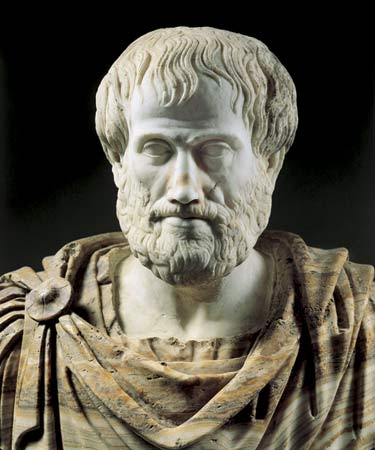
\includegraphics[scale=.5]{aristotle.jpg}
\end{center}
You can use 
\begin{itemize}
\item lists
\item like this
\end{itemize}
or numbered
\begin{enumerate}
\item like this,
\item or this
\end{enumerate}
but don't overdo it.

% This just dumps some pseudolatin in so you can see some text in place.
\blindtext

\chapter{My Second Content Chapter}
\label{chapterlabel3}



If you have a formal theorem you might try this.
% \begin{definition}\label{def}
% See definition~\ref{def}.
% \end{definition}
% \begin{theorem}
% For all $n\in\nats,\; 1^n=1$.
% \end{theorem}
% \begin{proof}
% By induction over $n$.
% \end{proof}

% This just dumps some pseudolatin in so you can see some text in place.
\blindtext

\chapter{Conclusions and Further Work}
\label{chapterlabel4}


\section{Conclusions}

At the start of this report we sought to address four questions in our problem formuation:

\begin{tight_enumerate}
    \item whether reasonable summaries can be generated from just lexical names in the function signature?
    \item whether reasonable summaries can be generated from the functions abstract syntax tree, without the lexical data?
    \item whether these models, can be combined in a way that surpasses each individually?
    \item whether such models can work both in an `in-project' setting and an `out-project setting'?
\end{tight_enumerate}

Over the course of this report we have provided evidence to address the answers to each of these questions. 

First we conclude that reasonable summaries \textit{can} be generated from just names in the function signature. 
In particular we have shown that reasonable descriptions can be generated from just the argument name, by looking at its the character substructure. Operating on our Reduced Random Split Dataset, our Seq2Seq model achieves test BLEU score of 12.72 - surpassing a Rote Learner that regurgitates memorised descriptions for similar names.  
We can also conclude that other aspects of the signature, such as corguments and the function name, also prove informative, since they boost perfomance in our Rote Learner and in most of our Seq2Seq cases. 
This highlights the informative power of the function signature, and the names that are chosen within it.

Secondly we conclude that reasonable summaries \textit{can} be generated from just the AST, without any reference to the name of the argument. 
By using the \textit{variable path-context} (VPC) representation, we showed that Rote Learner that memorised descriptions and matched VPCs could achieve a BLEU score of 12.61 on our Full Random-Split Dataset. This was then ourperformed by our neural Code2Vec Decoder, which achieved a test BLEU score of 18.13, generating original descriptions. 
We demonstrate that this model can outperform the Rote Learner despite partial or full occlusion of the names of objects in the AST, achieving BLEU scores of 16.94 and 13.07 respectively.

Thirdly we conclude that combining our two different modalities results in a stronger model than either of the two individually. By simply each individually concatenated encoded vectors our Code2Vec + Seq2Seq model surpasses individual models by 2 BLEU points on the Full Random-Split Dataset.

Finally our investigation to our the last question to proves inconclusive. We notice a significantly worse performance of our models on the `out-project' setting, though they generate sentences with fluency. We demonstrate that due to tokenizations of the dataset, a large fraction of test-set features are rendered out-of-vocabulary in this setting, raising the question of whether the models or the tokenizations are the problem in this case. 

% This just dumps some pseudolatin in so you can see some text in place.
\section{Limitations \& Critique}

In the course of the above investigations, we encountered a number of limitations that affected our progress.

\paragraph{Dataset} 
First and foremost, we noted that the composition of our dataset disproportionately originates from a single source - 41\% of our arguments are from \mintinline[]{python}{tensorflow}. This proved less problematic for Random Split Dataset but in a Library Split setting this accounts for most of the training data - which also includes \mintinline[]{python}{scipy} and \mintinline[]{python}{numpy}. Therefore the variance of our training set would have been much reduced, hindering our investigation into Library Split Data.

Secondly, although the size of our Full Datasets are comparable to others\footnote{such as the Stack Overflow SQL dataset}, our Reduced Dataset are arguably too small for our neural methods in character-level tasks. In particular this small dataset may explain the overfitting in these tasks, and should have ideally have been bigger in these investigations, or subject to data augmentation.

\paragraph{Metric} 
A major limitation of our overall investigation is a lack of automatic metrics for assessing description quality. Without skilled human intervention in reading the source code, it is hard to evaluate whether an argument description is true, even if the n-gram precisions (as measure by BLEU) is poor. In machine translation, often multiple synonymous reference sentences are provided to improve the validity of n-gram precision \citep{papineni_bleu_2001}, but in our case no multiple translations exist. Automating a measure of evaluating description would greatly assist in-depth analysis of where the models fail.

\paragraph{Resources} 

Finally a limitation of our overall investigation is our resources available. Since we aimed to fit all our work on one GPU, we were constrained to use a limited vocabulary of paths, terminal nodes. Increasing these would likely help in both Random Split and Library Split contexts

\section{Further Work}

* Seq2Seq
* 

\chapter{Note to Matko}
\label{baselines_note}

\textit{
This is a note to explain the current situation of the project, and to decide what might need doing in the last few weeks of the project. 
I'm aware I have a lot of different ways of chopping the data set, and differnet models, so there is potential to investigate a lot.
As such this note is just to clarify thoughts for this last week.}

\section{The Dataset (A Reminder)} % (fold)
\label{sec:the_dataset}

The raw dataset is the set of all functions that obey the \mintinline{python}{numpy} or \mintinline{python}{google} standard of docstrings, from top 300 libraries as available on \mintinline{python}{pip}. 
These were collected by writing an extension to the \mintinline{python}{sphinx} documentation generator, which is the industry standard for automatic code documentation.

In terms of the amount of data collected:
\begin{itemize}
    \item 133 libraries contributied to dataset
    \item 12,079 function definitions were collected
    \item 39,205 (argument, description) pairs were collected
\end{itemize}

In examining this data, I found the data to be highly biased towards scientific libraries, and also within these libraries, many functions containing identical pairs of (argument, description). 
The reasons for this are simple: 
\begin{enumerate}
    \item Scientific libraries have vast API's, so need good documentation for inputs and outputs.
    \item Some the arguments for these apis are likely to be identical, leading coders to copy them. 
    E.G \mintinline{python}{name} for a tensor in \mintinline{python}{tensorflow}.
\end{enumerate} 

\subsection{Data Set Investigation} % (fold)
\label{ssub:datasetinvestigation}

In the report I aim present an investigation of the dataset from a statistical point of view, but also a qualitative point of view.
I want to both know: 
\begin{itemize}
    \item Statistics about natural language: eg - variable names, description lengths, uniqueness of variable names and (variable, description) pairs, vocabulary size
    \item Statistics about code and syntax trees: eg - tree sizes, paths, uniquenesses of paths
    \item Clustering of natural language: eg how similar are the libraries? is there a distinction between scientific and other libraries, based on either description, or argument name, or names of source code. How much `bias' is there in the dataset?
\end{itemize}

I have done the first two investigations, on Jupyter notebooks but I am yet to do the third.

The results of the the first two investigations I will paste here fully in due time, but the in summary I noticed that there are a often arguments have identical descriptions, even if they come from different functions with different code. 
This allows a dumb learner that effectively just memorizes previous descriptions and names, to perform with  significant hit rate.  
As a result, I created various datasets that effectively capped the number of duplicate (argument, description) pairs.

\begin{center}
\begin{tabular}{|| c | c | c ||}
  \hline
   Name of DataSet & No of Duplicates & Data Set Size \\
  \hline
   UnsplitND1 & 0 & 22917 \\
   UnsplitND2 & 1 & 28771 \\
   UnsplitND3 & 2 & 31063 \\
   UnsplitND4 & 3 & 32487 \\
   UnsplitND5 & 4 & 33398 \\
   UnsplitNDX & 9 & 35551 \\
   Unsplit    & NA & 39205\\ 
  \hline
\end{tabular}
\end{center}

Finally I also had the option of choosing whether to divide my dataset along repository lines for training and validation/test, or whetehr to keep the function together. 
That is: should code from a the test and validation set be from different libraries as the train set. 

I have so far prepared one of these data sets but I have not prepared the no duplicates set.

\begin{center}
\begin{tabular}{|| c | c | c ||}
  \hline
   Name of DataSet & No of Duplicates & Data Set Size \\
  \hline
   Split    & NA & 39205\\ 
  \hline
\end{tabular}
\end{center}

\section{Hashtable Baselines} % (fold)
\label{sub:hashtable_baseline}

All hashtable baseline models shared a common idea: identify a feature to match, and randomly choose a stored description from the training set, whose data matches this feature. 
Although this led to several differnt models (largely based on what consitutes a match, and which features are available to the model), this baseline proved vital to compare to the LSTM models, as it indicated the limits of "overfitting". 
Surpassing these models should indicat that something generalizable in the data has been learnt.

\subsection{Natural Language Lookup} % (fold)
\label{sub:natural_language_lookup}
When dealing with natural language text data, the model attempted to find the largest overlapping n-character-gram, and drew randomly from the set of matched descriptions.

There were four available tokenizations of the data that only pertained to the natural language of the function signiature, and they were concatenated with unique character separators, to form long strings for the lookup table

% subsection natural_language_lookup (end)

\begin{enumerate}
    \item the argument name
    \item the argument name + the function name
    \item the argument name + the names of the other arguments
    \item the argument name + the function name + the names of the other arguments
\end{enumerate}

\subsection{Code Path Lookup} % (fold)
\label{sub:code_path_lookup}

In a similar spirit, the hashtable model aims to memorise `code paths' as defined in the code2vec paper, and then for each test point, return a randomly chosen description from the set of best matches.

In this case what constitutes a match can vary, so a delineation is based on whether full paths (`hard') need to be matched, or subpaths can be matched (`soft')
\begin{enumerate}
    \item \textit{hardest} - chose from the set of descriptions which have the most matching full paths.
    \item \textit{hard} - chose from the set of descriptions in proportion to the number of matching full paths.
    \item \textit{soft} - chose from the set of descriptions with the greatest matched subpaths.
    \item \textit{softest} - chose from the set of descriptions  with proportion to the number of matching subpaths.
\end{enumerate}

Of these, I run into memory issues with the soft (for some reason), and still need to run it on the full datasets. 
% subsection code_path_lookup (end)

\subsection{Combined Lookup} % (fold)
\label{sub:combined_lookup}

To do a combined lookup, simply add the two possible sets of descriptions together, before randomly choosing. 

% subsection combined_lookup_and_results (end)

\subsection{Results} % (fold)
\label{sub:results}

In terms of results, I first ran the hashtable baseline with just text and different tokenizations. If you remove the duplicates the model performs significantly worse.

Then I have on the same dataset run the code sections.

I found this.



\section{Neural Models} % (fold)
\label{sec:neural_models}

\subsection{CharToWord Seq to Seq} % (fold)
\label{sub:chartoword_seq_to_seq}

So far this model has failed to beat the baseline. At best it seems capable of matching it. My theories as to why this is:
 \begin{enumerate}
     \item Unlike in sentences where words depend on each other in a confusing syntactic patterns with long range dpependencies, words in a sentence have shorter range dependencies, often neighbouring matters the most or sub phrases.
     \item Therefore ngram overlap is a very significant feature - indeed its what humans look for when trying to work out what variables are
 \end{enumerate}

 I expected cases such as including functon name or other arguments to hurt performance, and it would add a lot of noise. This turned out not to be the case. Perhaps the benchmark's advantage of always being able to generate well formed descriptions also came into play.

 At any rate I have a significant number of experiments here, with the different tokenizations of the data, and different types of seq to seq model (attention no attention, bidirectional or not, trainable embeddings or not), that i could write about.

 \subsection{CodeToVec to Seq} % (fold)
 \label{sub:codetovec}

 This model is an implementation of thde code2vec paper 


 \subsection{To Do} % (fold)
 \label{sub:to_do}
 
 \begin{enumerate}
   \item split data set and run experiments
   \item rename variables in ast \& run (2 tokenizations)
   \item hyperparam sweep \& tune
   \item dropout for code 2 vec
   \item ?? use source code in bag of source code words model??
   \item use all paths (like code 2 vec paper)
   \item run hashtable baseline on other datasets
 \end{enumerate}
 % subsection to_do (end)
 









\chapter{Another Appendix About Things}
\label{appendixlabel2}
(things)

\chapter{Colophon}
\label{appendixlabel3}
\textit{This is a description of the tools you used to make your thesis. It helps people make future documents, reminds you, and looks good.}

\textit{(example)} This document was set in the Times Roman typeface using \LaTeX\ and Bib\TeX , composed with a text editor. 
 % description of document, e.g. type faces, TeX used, TeXmaker, packages and things used for figures. Like a computational details section.
% e.g. http://tex.stackexchange.com/questions/63468/what-is-best-way-to-mention-that-a-document-has-been-typeset-with-tex#63503

% Side note:
%http://tex.stackexchange.com/questions/1319/showcase-of-beautiful-typography-done-in-tex-friends 
  
% This line manually adds the Bibliography to the table of contents.
% The fact that \include is the last thing before this ensures that it
% is on a clear page, and adding it like this means that it doesn't
% get a chapter or appendix number.
\addcontentsline{toc}{chapter}{Bibliography}

% Actually generates your bibliography.
\bibliography{example}


% \appendix


\begin{thebibliography}{HHM99}


\bibitem[Pri70]{PriorNOP70}  %%only an example
A.~Prior.
\newblock The notion of the present.
\newblock {\em Studium Generale}, 23:  245--248, 1970.


\bibitem[Rey97]{Rey:D}
M.~Reynolds.
\newblock A decidable temporal logic of parallelism.
\newblock {\em Notre Dame Journal of Formal Logic}, 38(3):  419--436,
  1997.
\end{thebibliography}
\chapter{Other appendices, e.g. code listing}

\end{document}